\begin{frame}{What is missing data}
 \begin{itemize}
 \item Missing data happens when we intend to collect a piece of data but don't actually get it
 \item Historical approaches
 \begin{itemize}
  \item Complete Case analysis: Throw away any record that is not complete
  % list of downsides
 \item Available Case analysis: Use records so long as they are complete for the specific analysis in question
 %bad things here
 \end{itemize}
 \end{itemize}
\end{frame}


\begin{frame}{Imputation}
\begin{block}{Definition}
The English verb ``to impute'' comes from the Latin imputo, which means
to reckon, attribute, make account of, charge, ascribe. \cite{VanBuuren2012}
\end{block}
\begin{itemize}
 \item In the 1930's, Allan, Wishart,and Yates laid framework for missing data
 \begin{itemize}
  \item Idea: Fill in the missing value, deduct degrees of freedom to account for it
  \item Issue: Dogmatic, and variance can't be estimates correctly
 \end{itemize}

\end{itemize}

 
\end{frame}

\begin{frame}{Multiple Imputation}
Throughout the 70's and 80's Donald Rubin worked to improve on this
\begin{itemize}
 \item Instead of imputing one value, lets impute it $m\geq 2$ times
 \item Draw the values from the missing datas posterior distibution given the observed
 data and the process that generated the missing data
\end{itemize}
This idea is called Multiple Imputation (MI) and was formalized in 1987 \cite{Rubin1987}. It is the gold standard method
for missing data currently.
\end{frame}


\begin{frame}{How does MI work?}
 \begin{figure}[h!]
  \centering
    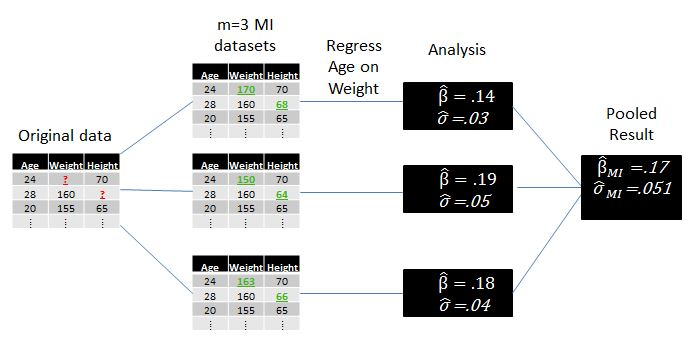
\includegraphics[width=0.8\textwidth]{mi_example_full.jpg}
  \caption{Visualization of MI data}
\label{fig:miexample}
\medskip
\small
Missingness is displayed by \textcolor{red}{?'s} and the imputed data is shown  as \textcolor{green}{\#'s}.
We then regress age on weight, get the results from the individual datasets, and then pool them together.
\end{figure}
\note{We will go in to much more detail later in presentation}
\end{frame}
